\documentclass[12pt]{article}
\usepackage{graphicx} % Required for inserting images
\usepackage{amsmath,amssymb,amsthm,amsfonts}
\usepackage{xcolor}
\usepackage{tasks}
%\usepackage{enumitem}
\usepackage[margin=1cm]{geometry}
\usepackage{tkz-euclide}
\usepackage{multicol}
\usepackage{pgfplots}
\pgfplotsset{compat=1.12}

\usepackage[utf8]{inputenc}
\usepackage[T1]{fontenc}
\usepackage{amsmath}
\usepackage{amsfonts}
\usepackage{amssymb}
\usepackage[version=4]{mhchem}
\usepackage{stmaryrd}
\usepackage{enumerate}
\usepackage{multicol}
\usepackage{xcolor}
\usepackage{graphicx}
\usepackage{ulem}
\usepackage{cancel}
\usepackage{tikz}
\usepackage{tkz-euclide}
\usepackage[finnish]{babel}

%\usepackage[style=alphabetic,]{biblatex}

%\usepackage[margin=2cm]{geometry}

\newcommand{\brac}[1]{\left(#1\right)}
\newcommand{\sqbrac}[1]{\left[#1\right]}
\newcommand{\set}[1]{\left\{#1\right\}}

\newcommand{\dd}[0]{\mathrm{d}}
\newcommand{\dx}[0]{\mathrm{d}x}

\newcommand{\hatu}{\hat{u}}
\newcommand{\hatv}{\hat{v}}
\newcommand{\hatw}{\hat{w}}
\newcommand{\hatn}{\hat{n}}

\newcommand{\vu}{\overline{u}}
\newcommand{\vv}{\overline{v}}
\newcommand{\vw}{\overline{w}}
\newcommand{\vp}{\overline{p}}
\newcommand{\vn}{\overline{n}}

\newcommand{\va}{\overline{a}}
\newcommand{\vb}{\overline{b}}
\newcommand{\vc}{\overline{c}}
\newcommand{\vd}{\overline{d}}


\newcommand{\vi}{\hat{\imath}}
\newcommand{\vj}{\hat{\jmath}}
\newcommand{\vk}{\hat{k}}

\newcommand{\ratkaisu}[1]{\hfill{\color{blue}\quad\textrm{Ratkaisu: } #1}}

\newcommand{\ratkaisuu}[1]{{\color{blue}\textrm{Ratkaisu: } #1}}

\newcommand{\kaava}[1]{{\color{green!50!black}#1}}

%\renewcommand{\ratkaisu}[1]{}
%\renewcommand{\ratkaisuu}[1]{}
%\renewcommand{\kaava}[1]{}

\newcommand{\vihje}[1]{{\color{red}Vihje. #1}}
\newcommand{\extra}[0]{\textbf{Extra.}~}

\title{OAMK}
\author{Juha-Matti Huusko}
\date{August 2023}

\renewcommand{\ratkaisu}[1]{{\color{blue}\quad\textrm{Ratkaisu: } #1}}

\renewcommand{\ratkaisu}[1]{}

\begin{document}
\thispagestyle{empty}

\begin{tikzpicture}[scale=0.8]
\foreach \y in {0,-1,...,-7} {
\draw (0,\y)--(10,\y);
}
\def\y{-1}
\foreach \x in {0,1,...,18} {
\draw (\x,\y) circle (2pt) node[above]{$\x$};
}
\draw (-1,\y) node[]{$x$};

\def\y{0}
\foreach \x in {0,10,...,100} {
\draw ({sqrt(\x)},\y) circle (2pt) node[above]{$\x$};
}
\draw (-1,\y) node[]{$x^2$};

\def\y{-3}
\foreach \x in {0,1,...,5} {
\draw ({exp(\x)},\y) circle (2pt) node[above]{$\x$};
}
\draw (-1,\y) node[]{$\ln(x)$};

\def\y{-2}
\foreach \x in {0,1,...,5} {
\draw ({2^(\x)},\y) circle (2pt) node[above]{$\x$};
}
\draw (-1,\y) node[]{$\log_2(x)$};

\def\y{-4}
\foreach \x in {0,1,...,2} {
\draw ({10^(\x)},\y) circle (2pt) node[above]{$\x$};
}
\draw (-1,\y) node[]{$\log_{10}(x)$};

\def\y{-5}
\foreach \x in {1,10,1000,10000} {
\draw ({ln(\x)},\y) circle (2pt) node[above]{$\x$};
}

\def\y{-6}
\foreach \x in {0,1,...,10} {
\draw[color=red] ({asin(\x/10)/10},\y) circle (2pt) node[above]{$\frac{\x}{10}$};
}
\draw (-1,\y) node[]{$\sin(x)$};

\def\y{-7}
\foreach \x in {0,1,...,10} {
\draw[color=red] ({acos(\x/10)/10},\y) circle (2pt) node[above]{$\frac{\x}{10}$};
}
\foreach \x in {1,2,...,8,9,10} {
\draw[color=red] ({18-acos(\x/10)/10},\y) circle (2pt) node[above]{$\frac{-\x}{10}$};
}
\draw (-1,\y) node[]{$\cos(x)$};

\end{tikzpicture}

\end{document}